\documentclass[7pt,landscape,a4paper]{scrartcl}   	

%Define which packages are used
\usepackage[landscape]{geometry} 		%Paper formatting
\usepackage{titlesec}
\usepackage{graphicx}	
\usepackage{multicol}				%Use for multiple collumns
\usepackage[ngerman]{babel}
\usepackage[utf8]{inputenc}
\usepackage{mathptmx}
\usepackage{listings}				%Used to display code
\usepackage{xcolor}
\usepackage{minted}
\usepackage{latexsym}				%Joins 

%Define Paper
\geometry{top=0.25cm,left=0.3cm,right=0.3cm,bottom=0.3cm} 
\setlength{\columnseprule}{1pt}
\graphicspath{ {./src/} }

%Define Color
\definecolor{green}{rgb}{0,0.6,0}
\definecolor{grey}{rgb}{0.89,0.89,0.89}
\definecolor{mauve}{RGB}{0,120, 255}
\definecolor{red}{RGB}{255, 0, 0}

%Define Code SQL
\lstset{frame=none,
	language={SQL},
	aboveskip=0.5mm,
	belowskip=0mm,
	showstringspaces=false,
	columns=flexible,
	basicstyle={},
	numbers=none,
	numberstyle=\footnotesize\color{gray},
	keywordstyle=\color{green},
	commentstyle=\color{red},
	stringstyle=\color{mauve},
	breaklines=true,
	breakatwhitespace=true,
	tabsize=4,
	backgroundcolor = \color{grey}
}

%define the section
\titleformat{\section}[block]
	{\normalfont\LARGE\bfseries}
	{}
	{0pt} 
	{\thesection.\space}
\titlespacing{\section}{0pt}{0.1ex}{0.1ex}

%define the subsection
\titleformat{\subsection}[block]
	{\normalfont\large\bfseries}
	{}
	{0pt}
	{\thesubsection\space}
\titlespacing*{\subsection}{0pt}{0.1ex}{0.1ex}

%define the subsubsection
\titleformat{\subsubsection}[block]
	{\normalfont\bfseries}
	{}
	{0pt}
	{\thesubsubsection\space}
\titlespacing*{\subsubsection}{0pt}{0.1ex}{0.1ex}

% -------------------------------------------------------------------------
\begin{document}
\begin{multicols*}{4}

% Title
\section{DBS - Marco Agostini}

%Grundlagen
\subsection{Grundlagen}
\textbf{Daten:} Maschinell verarbeitbar. \textbf{Informationen:} Sind interpretierte Daten.
Es gibt für formatierte und umformatierte Daten die passenden Systeme. \\
Ein \textbf{Datenbanksystem (DBS)} besteht aus \textbf{Datenbankmanagementsystem (DBMS)} und \textbf{1 bis n Datenbasen (DB)}. Die Datenstruktur wird im Datenkatalog(Data Dictionary) beschrieben und wird mit DDL erstellt. \\
\textbf{DBMS-Funktionen:} Speicherung, Transaktionen, Mehrbenutzerbetrieb, Sicherheit, Backup/Recovery, Datentypen, Abfragesprache, Programmierschnitstellen.\\
\textbf{Datenintegrität(Anf. DBMS)} 
\textit{Datenkonsistenz:} Logische Wiederspurchsfreiheit.
\textit{Datensicherheit:} Physische Sicherheit
\textit{Datenschutz:} Zugriffsschutz
%Datenbankmodelle
\subsection{Datenbankmodelle/Paradigmen}
Das Datenbankmodell legt die Datenstruktur fest, Strukturen im DBMS fest (Datentypen, Speicherung). \\
\textbf{Hierarchisches DBM:} Eine einzige Hierarchie, Beziehungen werden mit den Daten gespeichert. Nachteile: Die Welt ist nicht hierarchisch, Keine Trennung zwischen internen und externem Schema, aufwendige Anpassungsarbeiten.\\
\textbf{Netzwerk DBM: } Vernetzte Hierarchien, Beziehungen werden in einer Hierarchie gespeichert. Nachteile: Effiziente Anwendung war möglich mit der Kenntnis der komplexen Netzwerk-Datenstruktur.\\
\textbf{Relationales DBM:} Alle Informationen werde als unstrukturierte Daten (1.NF) gespeichert. Sehr flexibel. Klare und genaue Trennung zwischen Daten und Anwendungen. Nachteile: Independence Missmacht: Zwischen Typensystem der Programmiersprache und den Tabellenstrukturen. Komplexe Abfragen führen zu Performance-Problemen.\\
\textbf{Objektrelationales DBM:} Erweiterung des rel. Datenmodelles. (benutzerdef: Typen, Tabellen, Vererbung). Verschachteln von Tabellen (1. NF nicht nötig) Neben Daten (Objekte, Attribute) auch Methoden speicherbar.
%Entwurfsprozess
\subsection{Entwurfsprozess}
\textbf{Generalisierung/Spezialisierung} Ein Angestellter kann mehrere Rollen haben. is-a Beziehung. \textit{Abstrakte Basisklasse: } Legt Kontrakt für Basisklasse fest, kann nicht installiert werden. \textit{disjoint:} Objekt ist Instanz einer Unterklasse. \textit{overlapping:} Objekt kann Instanz von mehreren überlappenden Unterklassen sein. \textit{complete:} Alle Subklassen sind definiert. \textit{incomplete:} nicht-vollständig: Zusätzliche Subklassen sind erlaubt.\\
\textbf{ANSI-3-Ebenen-Modell}\\
\textbf{Externe Ebene:} Sicht einer Benutzerklasse auf Teilmenge. (Externes Schema). \\
\textbf{Logische Ebene:} Logische Struktur der Daten. (Logisches Schema). \\
\textbf{Interne Ebene:}  Speicherstrukturen (Internes Schema). \\
\textbf{Mapping:} Zwischen den Ebenen ist eine oder mehrere komplexe Abbildungen notwendig.
\subsubsection{Datenmodellierung}
Der konzeptuelle Entwurf wird mit UML realisiert. Der logische Entwurf wird mit der relationalen Schreibweise definiert.\\
%Konzeptzuelles DM
\textbf{Konzeptuelles Datenmodell}
Definiert die Daten-Objekte und deren Eigenschaften, Zusammenhänge und Beziehungen, legt Konsistenzbedingungen fest. Ist Lösungs- und Technologieabhängig. (UML/ER)\\
\textbf{Logischer DB-Entwurf} \textit{Schritt 1.} Abbildung des Konzeptuellen Modells (Domain Model) in das relationale Model. \textit{Schritt 2.} Überprüfen der Konsistenz des rel. Modelle. (Normalenformen)
\subsubsection{Relationales Datenmodell}
Mathematisches Konzept. Benutzt Tabellen zur Darstellung von Daten und Beziehungen.\\
\textbf{Regeln für die Abbildung: }Saubere Trennung zwischen der logischen und internen Schicht. Tabellen und Attribute in Gross-und-Kleinschreibweise.\\
\textbf{PS} werden unterstrichen.  \textbf{Fremdschlüssel} werden kursiv gschrieben mit REFERENCES TabelleA. 
\textbf{Schlüsselkandidaten-Attribute} sind mit UNIQUE auszuzeichnen. Attribute sind default: NOT UNIQUE, NULL\\
 \textbf{Schlüssel:} Attribut oder Kombination von Attributen, das/die ein Tupel eindeutig identifizieren. Die Kombination muss minimal sein. Eigenschaften: Eindeutig, Laufend Zuteilbar, kurz, invariant.\\
\textbf{Sekundärschlüssel:} Alternativer Suchschlüssel, nicht unbedingt eindeutig. \\
\textbf{Surrogatsschlüssel:} Künstlicher Schlüssel, der als Primärschlüssel verwendet wird.
\subsubsection{Normalenformen}
\textbf{Änderungsanomalie:} Änderung muss an mehreren Orten vollzogen werde. \\
\textbf{Einfüganomalie:} Tupel kann erst hinzugefügt werden, wenn andere Tupel existieren. \\
\textbf{Löschanomalie} Wenn ein Tupel gelöscht wird, gehen weitere Informationen verloren. \\
\textbf{Mutationsanomalie} Andere Tupel werden geändert.\\
\textbf{1. Normalenform} Wertbereiche der Attribute sind atomar.\\
\textbf{2. Normalenform} Jedes Nichtschlüsselattribut voll funktional abhängig von jedem Schlüsselkandidaten.\\
\textbf{3. Normalenform} Kein Nichtschlüsselattribut transitiv abhängig ist von einem Schlüsselattribut.
%Abbildungsregeln
\subsection{Abbildungsregeln in Logisches Modell}
Das konzeptuelle Model (Domain Model) wird in das logische Modell (relationale Schreibweise) abgebildet.
\subsubsection{Regel 1. Abbildung von Klassen}
Jede Klasse wird auf eine Tabelle abgebildet.
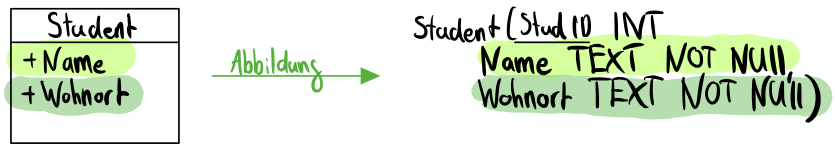
\includegraphics[width=0.85\linewidth]{regel1}
\subsubsection{Regel 2.1 vorausgesetzt (1...n)}
Assoziation mit Kardinalität (1...*). Der Primärschlüssel muss in der zweiten Tabelle als Fremdschlüssel vorkommen. Sprich das Objekt braucht eine Beziehung. (FS NOT NULL)
\subsubsection{Regel 2.2 I optionale AS mit FS NULL (0...1 zu 0...*)}
Wie 2.1 mit optionalen Beziehungsattributen. Mit NULL-Werten für nicht vorhandene Beziehungen. (FS NULL) Für häufig vorkommende Beziehungen.
\subsubsection{Regel 2.2 II optionale AS mit Beziehungstabelle (0...1 zu 0...*)}
Mit separater, abhängiger Beziehungstabelle (Zwei FS + Attribute) für seltene Beziehungen. (kanonische Lösung)
\subsubsection{Regel 2.3 Abbildung von Aggregationen}
\textbf{A)} starke Ganzes-Teile-Beziehung (Komposition, abhängige Tabelle PS/FS ref. PS)\\
\textbf{B)} schwache Ganzes-Teile-Beziehung (Aggregation, Beide haben PS)
\subsubsection{Regel 2.4 n:m}
Wird mit einer abhängigen Beziehungs-Tabelle mit Zusammengesetzen Primärschlüsseln moderiert. \\
\textbf{A)} Beziehungsklasse (PS = beide FS) (- Zusammengesetzte Schlüssel können sich fortpflanzen)\\
\textbf{B)} Assoziative Klasse aus (PS + zwei FS) (- Unique Contstraint)
\subsubsection{Regel 3}
\textbf{A) 1:1 Abbildung aller Tabellen} Die Superklasse wird auf einte Tabelle abgebildet mit einem Attribut, welches den Typ der Subklasse spezifiziert. (+ Flexibel und Redundantzfrei - Viele Tabellen, Komplexer Zugriff)\\
\textbf{B) Eine alleinstehende Tabelle pro Subklasse}
 Jede Subklasse erhält eine eigene Tabelle und enthält alle Attribute. (+ Einfacher Zugriff - Semantikverlusst, Schlüssel-Eindeutigkeit (Kontrolle über mehrere Tabellen), Modulation, keine überlappende Vererbung möglich)\\
\textbf{C) Eine Superklasse}
Die Superklasse erhaltet alle Attribute auch die der Subklassen mit einem diskriminierenden Attribut. (+ Einfache Zugriffe - Viele NULL Werte, 3. oder höhere Normalenform verletzt)
\subsection{Relationale Algebra}
Definiert Operationen, die sich auf eine Menge von Relationen anwenden lassen.\\
%Selektion
\begin{minipage}[b]{0,5\linewidth}
\begin{lstlisting}{SQL}
SELECT * FROM mitarbeiter
WHERE gehalt > 50;
SELECT a1, a2 FROM TABLE;
SELECT * FROM t1, t2;
\end{lstlisting}
\end{minipage}
\begin{minipage}[b]{0,5\linewidth}
Selektion $[\sigma]$\\
$\sigma_{(gehalt>50)}mitarbeiter$\\
Projektion $[\Pi]$\\
Kartesisches Produkt $[x]$
\end{minipage}
%SQL DDL
\section{SQL}
\subsection{SQL Data Definition Language}
\begin{lstlisting}[language=SQL]
CREATE DATABASE foo WITH OWNER = 'bar';
CREATE INDEX indexname ON tbl_name (attribute);
\end{lstlisting}
\begin{lstlisting}[language=SQL]
CREATE TABLE person (
	persnr INTEGER PRIMARY KEY, -- Collumn Constraint
	vorname VARCHAR(20) NOT NULL,
	name VARCHAR(20) NOT NULL,
	geburtsdatum DATE,
	-- Table Constraint
	PRIMARY KEY (persnr)
);
\end{lstlisting}
\subsubsection{Referentielle Integrität}

\begin{lstlisting}[language=SQL]
ON DELETE CASCADE --Tupel mit FS werden geloescht
ON DELETE RESTRICT --Tupel mit Ref. werden blockiert
ON DELETE SET NULL --Tupel mit FS werden NULL
ON DELETE SET DEFAULT --Tupel mit FS werden Default
\end{lstlisting}
\subsection{SQL Data Manipulation Language}
\begin{lstlisting}{SQL}
INSERT INTO tablename VALUES (23, 'Volkswagen');
INSERT INTO tablename(name, abtnr)
	VALUES('Entwicklung', 20);
\end{lstlisting}
\begin{lstlisting}{SQL}
UPDATE abteilung SET name='Verkauf' WHERE abtnr=3;
DELETE FROM abteilung WHERE abtnr=21;
\end{lstlisting}
\textbf{Selektion} \\
Mit dem Like kann nach String-Mustern gesucht werden:\\
 (\% 0 bis n Zeichen,\_ ein Zeichen) 
\begin{lstlisting}{SQL}
SELECT DISTINCT wohnort, name FROM angestellter
WHERE abtnr=3 AND name LIKE '%marc%'
ORDER BY wohnort ASC;
\end{lstlisting}
\textbf{Aggregatsfunktionen}
Null-Werte werden bei Aggregatsfunktionen übersprungen. Wird oft mit GROUP BY kombiniert. Die Having Klausel darf nur nach GROUP BY Verwendet werden.
\begin{lstlisting}{SQL}
[MIN | MAX | AVG | SUM | COUNT | FIRST]
SELECT AVG(salaer) FROM angestellter
GROUP BY abntnr;
\end{lstlisting}
\subsection{Joins $\Join$}
\textbf{Inner Join:} Filtern der Zeilen
\begin{lstlisting}{SQL}
SELECT abt.name, ang.name FROM
abteilung INNER JOIN angestellter
ON abt.abtnr=ang.abtnr;
\end{lstlisting}
\textbf{Left Outer Join:} Lässt Werte von Links stehen
\begin{lstlisting}{SQL}
SELECT a.attr, b.attr FROM tablename t1
LEFT OUTER JOIN tablename2 t2
ON t1.attr = t2.attr;
\end{lstlisting}
\textbf{Equi Join:} Tabelle joint sich selbest verknüpft
\textbf{Natural Join:} Join nach gleichen Attributen.\\
\textbf{Theta Join: } Kartesische Produkt + JOIN-Bedingung
\subsection{Mengenoperatoren}
Anhahl und Typ der Felder muss übereinstimmen. 
\begin{lstlisting}{SQL}
[ UNION | UNION ALL | INTERSECT | MINUS | EXCEPT]
SELECT persnr, name
FROM angestellter 
UNION
SELECT projnr, bezeichnung 
FROM projekt
ORDER BY 1;
\end{lstlisting}
\subsection{Unterabfragen}
Für jeden Tupel wird die Unterabfrage ausgewertet. EXISTS = Boolean!
\begin{lstlisting}{SQL}
[NOT IN | EXISTS | NOT EXISTS | ANY | ALL]
SELECT ang.name, ang.salaer FROM angestellter ang
INNER JOIN abteilung abt ON ang.abtnr=abt.abtnr
WHERE abt.name='Marketing'
AND ang.salaer < ALL
(	SELECT salaer FROM angestellter ang1 
	INNER JOIN abteilung abt1
	ON ang1.abtnr=abt1.abtnr
	WHERE abt1.name='Entwicklung'
);
\end{lstlisting}
\subsection{Modern SQL}
\textbf{Window Functions}
Funktionen, die auf ein Datenfenster angewendet werden. Mächtiger als GROUP BY. Tupel werden beibehalten, aber extra Spalte wird angehängt.
\begin{lstlisting}{SQL}
SELECT persnr, abtnr, max(salaer) OVER (PARTITION BY abtnr) 
FROM angestellter;
\end{lstlisting}
\textbf{Common Table Expressions}
Ermöglichen Hilf-Queries in bzw. von einer grösseren Query. Sind temporäre Tabellen.
\begin{lstlisting}{SQL}
WITH sometable1 AS (
	SELECT * from sometable2;
),
sometable2 AS (
	SELECT * FROM sometable1
), 
SELECT * FROM sometable2;
\end{lstlisting}
Rekursive Variante
\begin{lstlisting}{SQL}
WITH RECURSIVE unter ( name, persnr, chef) AS
	(SELECT A.name, A.persnr, A.chef FROM angestellter A
 	WHERE A.chef = 1010
  	UNION ALL
	SELECT A.name, A.persnr, A.chef FROM angestellter A
  	INNER JOIN unter B ON B.persnr = A.chef
) SELECT * from unter;
\end{lstlisting}
\textbf{Lateral Joins}
Query mit dem Inhalt einer anderen Tabelle ergänzen. Tabellen haben ohne Lateral keinen Zugriff auf Attribute anderer Tabellen. Die 
\begin{lstlisting}{SQL}
SELECT abt.abtnr, ang.persnr, ang.name, ang.salaer
FROM abteilung AS abt
JOIN LATERAL (
	SELECT * 
	FROM angestellter
	WHERE abt.abtnr = angestellter.abtnr
	ORDER BY salaer DESC
	LIMIT 3
) ang ON true;
\end{lstlisting}
\subsection{Views}
Datenkapselung auf interner Ebene. Vereinfachung der Abfrage. 
Sicherheit: irrelevante Daten werden verborgen. Virtuelle Tabelle basierend auf Tabellen oder Views. \\\textit{Materialized View:} existieren in Tabellenform und werden nicht automatisch aktualisiert.
\begin{lstlisting}{SQL}
CREATE VIEW name (persnr, name, tel) AS
	SELECT	persnr, name, tel 
	FROM angestellter;
\end{lstlisting}
\subsection{Datenbanksicherheit}
\textbf{Systemsicherheit:} Identifizierung, Autorisierung von Benutzern. Kontrolle der System-Ressourcen. Auditing. Kommunikationssicherung.\\
\textbf{SQL Injection}
Angreifer erstellt SQL-Kommandos oder verändert existierende um versteckte Daten sichtbar zu machen, Daten zu überschreiben oder auf Systemebene des Hosts zu gelangen. \textit{Massnahmen:} Input prüfen, Datenzugriff abstrahieren, Benutzerverwaltung.\\
\textbf{Benutzerverwaltung / SQL Data Control Language}
Jeder Nutzer erhält System- und Datenprivilegien. Rollen erhalten diese Rechte. (Rollen = Gruppen und Benutzer)
\begin{lstlisting}{SQL}
CREATE ROLE user_name
WITH LOGIN PASSWORD 'passw0rd';
GRANT INSERT ON TABLE angestellter to user_name;
REVOKE UPDATE on angestellter from user_name;
\end{lstlisting}
\textbf{Row-Security} Ermöglich Zugriff auf eine Untermenge von Zeilen einer. Tabelle.
\subsection{Transaktionen}
Höhere Geschwindigkeiten durch Verzahnung/Paralelität mit korrekter Isolation. 
\subsubsection{ACID}
\textbf{Atomicity:} Eine Transaktion wird nur vollständig durchgeführt.\\ \textbf{Consistency:} Die Daten werden von einem Konsistenten Zustand in den nächsten gebrach. \textbf{Isolation:} Eine Transaktion soll so ausgeführt werden, als sei sie isoliert. \textbf{Durability:} Alle Änderungen einer Transaktion sind persistent und gehen nicht durch Fehler verloren.
\begin{lstlisting}{SQL}
BEGIN TRANSACTION;
SAVEPOINT firstsavp;
ROLLBACK TO SAVEPOINT firstsavp;
COMMIT TRANSACTION;
\end{lstlisting}
\subsection{Isolation}
\textbf{Serialisierbarkeit} 
Nebenläufigkeit, soweit das Ergebnis equivalent zur seriellen Ausführung ist. Ziel ist es zyklischen Informationsfluss sicherzustellen.\\
\textit{Formalisierung} \\
r$_{a}$(x) Transaktion T$_{a}$ liest DB-Objekt x\\
w$_{a}$(x) Transaktion T$_{a}$ schreibt DB-Objekt x\\
c$_{a}$(x) Transaktion T$_{a}$ ruft Commit auf\\
\textbf{Serialisierbarkeitsgraph}\\
Jedes Konfliktpaar symbolisiert eine Verbindung zwischen den Transaktionen. 1. Konfliktpaare bestimmen 2. Graph zeichnen und analysieren. \textit{Zyklenfrei $<=>$ Serialisierbar}\\
Commit nur möglich, falls keine Konfliktpaare einer anderen Transaktion folgen.\\
\textbf{Pessimistische Locking Verfahren}\\
\textit{Exclusive Lock (x)}\\
Read/Write. Nur eine Transaktion kann den Lock erhalten.\\
\textit{Shared Lock (s)}\\
Read. Mehrere Transaktionen können den Lock erhalten.\\
\textit{Granularität}\\
Locks können Salbe, Table Ranges, Rows, Item erhalten. (Meistens auf der Row)\\
\textbf{Two-Phase-Locking 2PL}\\
Zwei Phasen: Growing und Shrinking Phase. Sobald ein Lock freigegeben wird, das sie nichts neues Locken. Probleme: Cascading Rollbacks, Deadlocks. (Behoben durch time out oder Abbruch einzelner Transaktionen.)\\
\textbf{Strict Two-Phase-Locking S2PL}\\
Alle gehaltenen Locks werden erst am Ende der Transaktion freigegeben.  
Probleme: Deadlocks möglich. (Kein Cascading Rollback, kein unklarer Beginn der Shrinking  Phase)\\
\textbf{Preclaiming Two-Phase-Locking}\\
Transaktion muss alle Locks auf einmal (atomar) am Anfang belegen. Dies garantiert die Deadlock-freiheit. Nicht realistisch umsetzbar!
\subsection{Isolation-Levels}
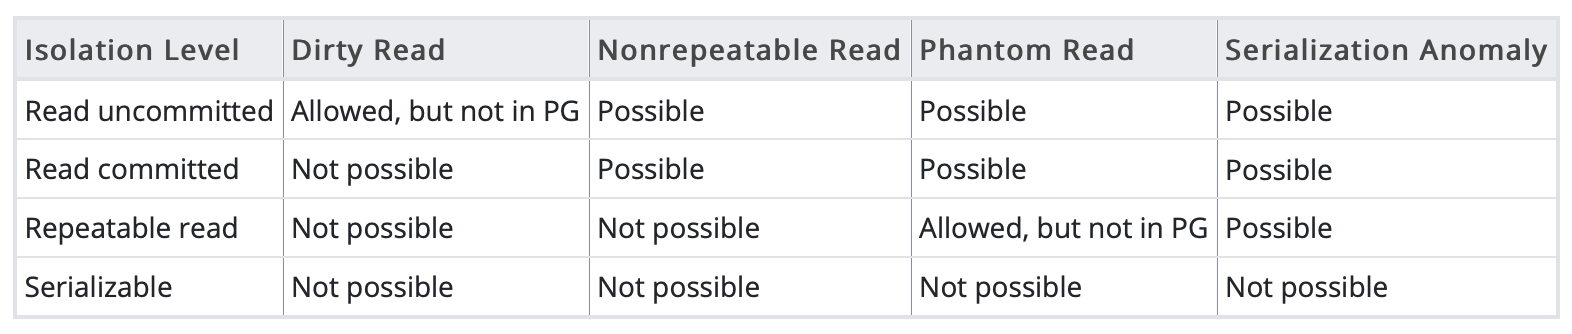
\includegraphics[width=\linewidth]{isolationlevels}
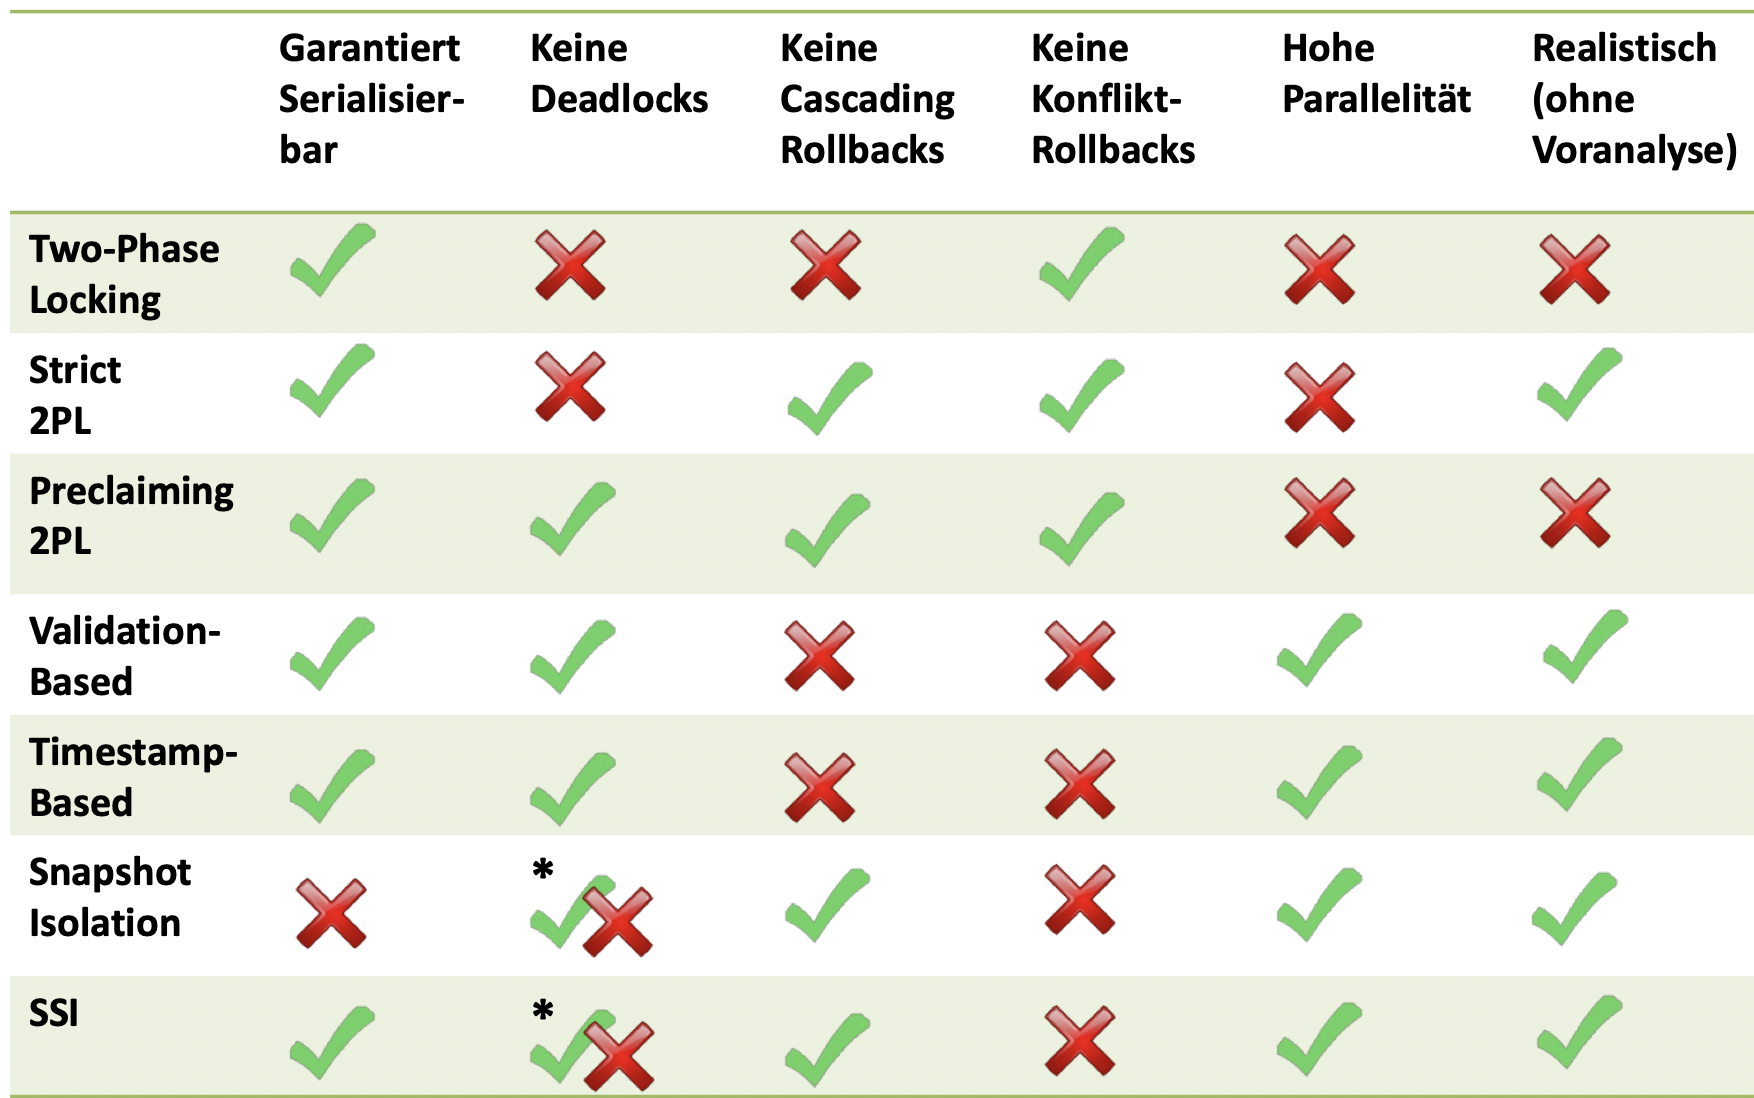
\includegraphics[width=0.5\linewidth]{isolation}\\
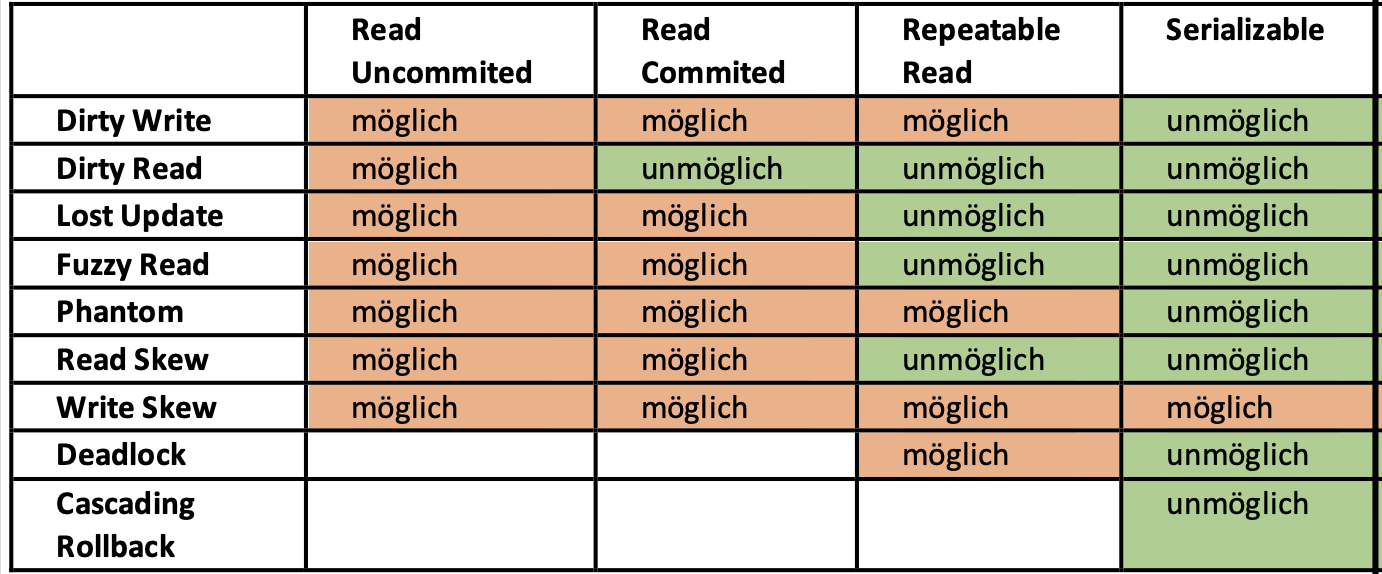
\includegraphics[width=0.75\linewidth]{locks}\\
Das Isolations-Level Serializable ist die richtige vollständige Isolation nach ACID.\\
\textbf{Read Uncomitted:} Lesezugriffe werden nicht synchronisiert.\\
\textbf{Read Commited:} Lesezugriffe werden kurz/temporär synchronisiert.\\
\textbf{Repeatable Read:} Einzeln zugegriffen Rows werden synchronisiert. (SI/MVCC)\\
\textbf{Serializable:} Vollständig korrekte Isolation. (SSI)
%-------------------
\subsubsection{Fehlertypen}
\textbf{Dirty Read: } Liest Daten von anderer abgebrochenen Transaktion. \\
\textbf{Non-Repeatable Read (Fuzzy Read): } Liest Daten mehrmals und sieht andere Werte.\\
\textbf{Phantom Read:} Suchkriterien treffen während einer Transaktion auf unterschiedliche Datensätze zu, weil eine andere Transaktion Datensätze hinzugefügt oder entfernt hat.

\subsubsection{Optimistische Verfahren}
\textbf{Snapshot Isolation SI}\\
 Jede Transaktion sieht Snapshot zu seinem Start-Zeitpunkt. Bei Commit wird geprüft, ob Objekte noch unverändert wie bei Start sonst rollback. Erfüllt Serializable nicht. Lässt Write Skew-Anomalie und Read-only transaction Anomalie zu. (Lesen blockiert schreiben, schreiben blockiert lesen nicht)\\
\textbf{MVCC Multi-Version Concurrency Control}\\
Realisiert SI. Intern werden verschiedene Versionen eines Objektes gehalten, die durch Zeitstempel oder Transaktionsnummer voneinander unterschieden werden. Bei Update werden Tupel mit x-lock versehen - Deadlocks möglich. Beim Lesen werden keine Locks gesetzt bzw. überprüft. (Schreiber/Leser blockieren keine Leser, Schreiben blockieren Schreiber)
\subsection{Architektur}
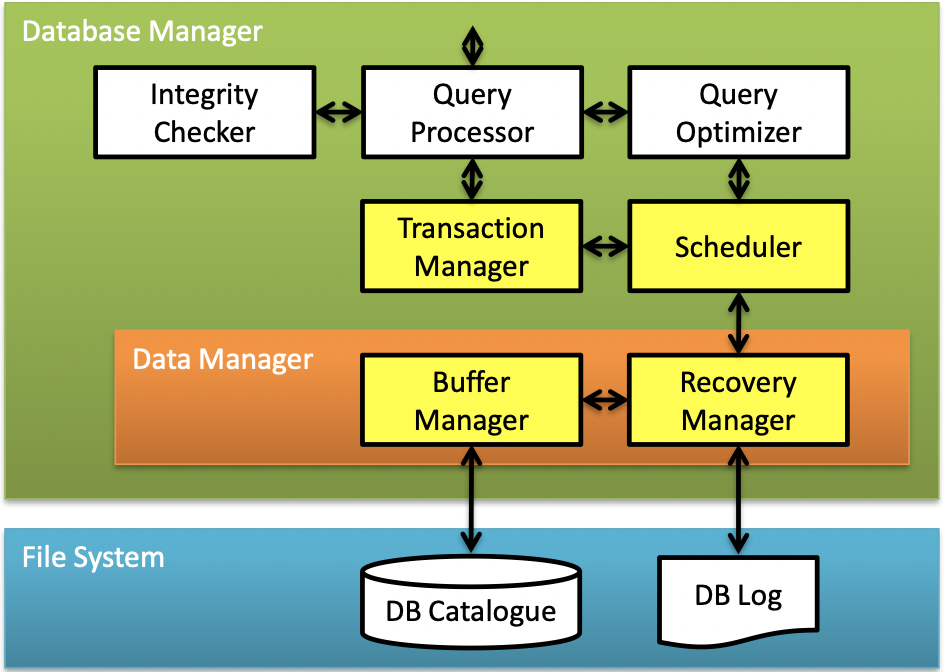
\includegraphics[width=0.75\linewidth]{architektur}
\begin{minipage}[b]{0,24\linewidth}
\textbf{Dateien DBMS}
\textbf{Logisch} Sammlung von Datenwerten\\
\textbf{Abstrakt physisch} Folge von Datenblöcken\\
\textbf{Physikalisch} Sammlung von Sektoren.\\
Pages in Blöcken abstrahiert.\\
\end{minipage}
\textbf{Transaction-Manger} koordiniert die Transaktionen und kommuniziert mit dem Scheduler.\\
\textbf{Der Scheduler} Ist für die Koordination der parallele laufenden Transaktionen zuständig. \\
\textbf{Recovery-Manager} Muss bei Abbruch einer Transaktion die Daten wieder in einen konsistenten Zustand zurückführen.\\
\textbf{Buffer-Manager} Verwaltet den internen DB-Puffer. Stellt mit Storage-Manger den Transfer zwischen Haupt- und Sekundärspeicher sicher.\\
\textbf{Planer/Optimizer}\\
Erzeugung eines optimalen Ausführungsplanes (Execution Plan). Wählt alle möglichen Ausführungspläne und wählt denjenigen, der am günstigsten ist. 
\subsection{Fehlerklassifikation}
\textbf{Fehler einer Transaktion} Ursachen: Fehler in der Applikation-SW, Abbruch einer Transaktion durch Applikation oder System (Deadlock-Auflösung). Inkonsistenz: Festgeschriebene Änderungen Recovery: Rollback oder lokales undo. (Millisekunden)\\
\textbf{Hauptspeicherverlust} Ursachen: Fehler in der DB-System-SW, HW-Fehler, Stromausfall. Inkonsistenz: Verlust von Änderungen, die noch nicht auf die Disk geschriben wurden. Recovery: Gloabes Undo: alle aktiven Transaktionen zurücksetzen.\\
\textbf{Hintergrundspeicherverlust} Ursachen: Fehler im Disk-Treiber, Feuer, Wasser etc. 
Inconsistent: Verlust der Daten auf der Disk. Recovery: Rekonstruktion der verlorenen Daten, Backup und Log-File-Techniken.
\subsection{Log-Files}
\textbf{Write-Ahead-Log WAL}\\
$[ LSN, TransactionID, PageID, Redo, Undo, PrevLSN]$\\
$[\#2, T_{1}, P_{A}, A=250, A=200, \#1]$\\
$[\#3, T_{2}, P_{C}, C=100, C=150, \#2]$\\
Gewährleistung (AC). Modifikationen werden vor dem eigentlichen Schreiben protokolliert.\\
\textbf{Log Sequence Number:} Eindeutig, monoton ansteigend\\
\textbf{TransaktionsID:} Transaktionskennung der Transaktion\\
\textbf{Page:} Kennung der Page der Änderung\\
\textbf{Redo:} Gibt and, wie die Änderung nachvollzogen werden kann. Absoluter Wert nach der Änderung.\\
\textbf{Undo:} Gibt an, wie die Änderung rückgängig gemacht werden kann. Absoluter Wert nach der Änderung.\\
\textbf{PrevLSN:} Zeiger auf den vorhergehenden Log-Eintrag.\\
\textbf{Wiederanlauf nach Fehler}\\
\textbf{Winners - REDO}\\
Transkationen, die nach dem letzten Checkpoint duchgeführt wurden.\\
\textbf{Loosers - UNDO}\\
Transaktionen, die zum Zeitpunkt des Absturzes noch aktiv Waren.
\subsection{Index-Strukturen}
Selbständige Datenstruktur, redundant zur Tabelle. Beschleunigt den Lese-Zugriff auf Kosten INSERT/UPDATE/DELETE.\\
\textit{Zwei Strukturen:} Data Pages (Heap) - Linked-List der Daten.
Suchbaum - Indexeinträges (Nodes,Leaves)
\\
\textbf{Index-Sequential Access Method ISAM}\\
+ Einfügen, Suchen / - Aktualisieren\\
Daten werden über die indesxspalte aufsteigend sortiert. Grösster Schlüsselindex im Block wird vermehrt und in den Index gelegt. Sehr dünner Index mit logischen Adressen.\\
\textbf{B-Bäume}\\
+ Lesen Schreiben\\
Balancierte Mehrwege Suchbäume. Geeignet für Hintergrundspeicher. \\
\textbf{B+-Bäume}\\
Nur Blätter/Leaves enthalten Daten. Blätter sind verkettet (Linked-List). Die Verkettung erlaubt eine schneller Interation. \\
\textbf{Hash} 
Ordnet Key den Einträgen zu.
Problem: Overflow.\\
\textbf{Zusammengesetzter Index}
\begin{lstlisting}{SQL}
CREATE INDEX mytable_col12_idx
ON mytable (col1, col2);
\end{lstlisting}
\textbf{Partieller Index}
\begin{lstlisting}{SQL}
CREATE INDEX mytable_col_part_idx
ON mytable (col)
WHERE archived IS NOT NULL;
\end{lstlisting}
\textbf{Funktionaler Index}
\begin{lstlisting}{SQL}
CREATE INDEX mytable_col_part_idx
ON mytable (immutable_function (col)); --upper, lower
\end{lstlisting}
\textbf{Index mit INCLUDE}
\begin{lstlisting}{SQL}
CREATE INDEX magic_idx
ON test (nr,id) INCLUDE (txt);
\end{lstlisting}
\subsection{Optimierung}
Die syntaktische/lexikalische Reihenfolge der Klauseln entspricht nicht der logischen Reihenfolge der Operationen und auch nicht der effektiven.\\
\textbf{Übersetzen einer SQL-Abfrage}\\
1. SQL parsen und in Baumstruktur abbilden\\
2. Query validieren\\
3. Views auflösen\\
4. Query Optimieren\\
5. Execution Plan erzeugen\\
6. Code erzeugen bzw. ausführen\\
7. Resultat in Query ausgeben\\ 
\textbf{Logische Optimierung}\\
Abfrage so umformulieren, dass sie dasselbe Resultat liefert, aber effizienter berechnet werden kann.\\
Selektion so früh wie möglich, um die Zwischenergebnisse so klein wie möglich zu halten. \\
\textbf{Physische Optimierung}\\
Effiziente Algorithmen wählen, um die Operationen der relationale Algebra zu implementieren.Kostenbasierte Auswahl aus einer Menge von Plänen.
Kosten sind u.a. von den verfügbaren Plänen abhängig. \\
\textbf{Ausführungspläne} Kommunikationskosten, Berechnungskosten, I/O-Kosten, Speicherkosten.\\
\textbf{Statistiken} Informationen über Relationen und Indexe in Systemkatalog verwaltet. (Je nach DBMS nur periodisch aktualisiert.\\
\textbf{Der Planner}\\
Der Planner beginnt bei der Generierung bei den Relationen (Tabellen) der Query. \textit{Full Taube Scan / Seq Scan} Scannt den ganzen Table. \textit{Index Scan} Falls es ein Attribut gibt, nach dem gefiltert werden kann.  Bei kleineren Datenmengen aus dem selben Disk-Block ist ein Seq Scan Scheller als ein Index-Scan. Lädt einen Tutel-Zeiger nach dem andere aus dem Index und greift sofort auf das entsprechende Element ind er Tabelle zu. \textit{Bitmap Index/Heap scan} Lädt alle Tutel-Zeiger auf einmal aus dem Index, erzeugt ad-hoc einen internen Bitmap-Index, um sie dann im Hauptspeicher zu sortieren und lädt alle Tabellen-Tupeln.\\
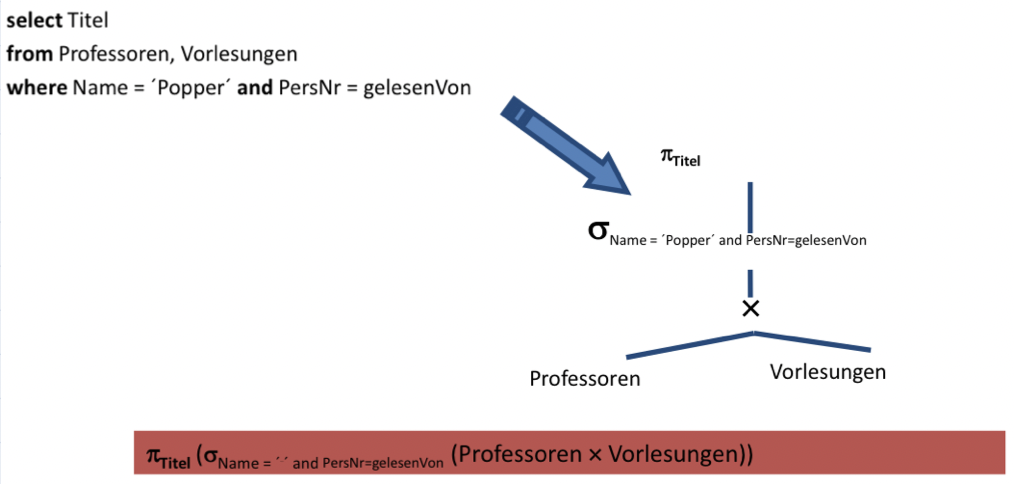
\includegraphics[width=\linewidth]{optimierung}\\
\textbf{VACUUM}\\
Bei MVCC entsteht eine Tupel-Kopie pro Transaktion. Diese Tupel werden nach Transaktionsabschluss als gelöscht markiert - jedoch nicht gelöscht. VACUUM ist eine Art Garbage-Collection als Hintergrundprozess und aktualisiert die Statistik. Verwendet keinen Locks und kann im Betrieb ausgeführt werden. (VACUUM FULL verwendet locks)
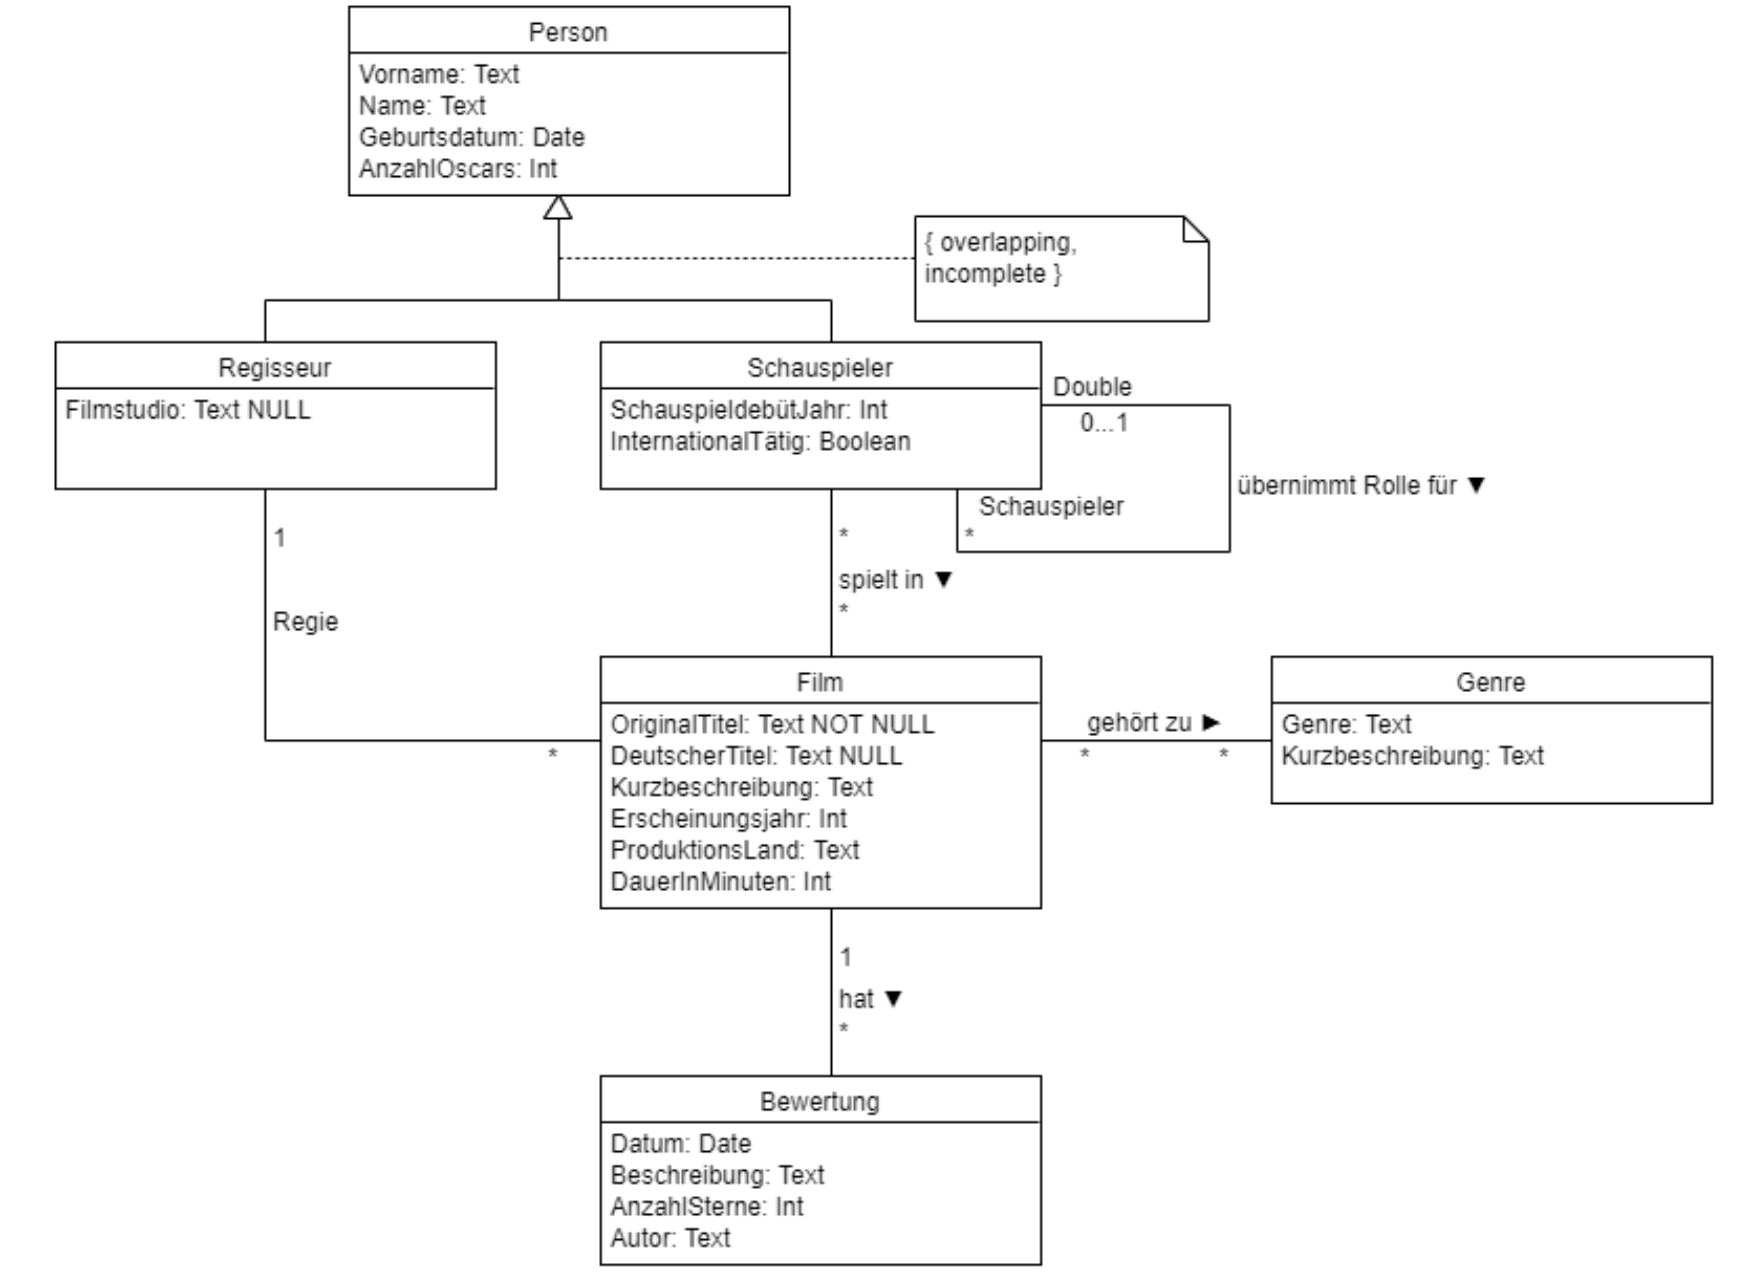
\includegraphics[width=\linewidth]{uml}
\textbf{Logisches Modell}\\
bewertung (\\
\underline{id} INTEGER,\\
datum DATE,\\
beschreibung TEXT, \\
anzahlSterne SMALLINT,\\
autor TEXT,\\
\textit{film} NOT NULL REFERENCES film
);

\end{multicols*}
\end{document}